\clearpage
\appendix
\section*{Supplementary Material}
\addcontentsline{toc}{section}{Supplementary Material}

Every number reported here is drawn from the same runs as the main paper. Nothing
in this appendix revises a result in Section~\ref{sec:results}; the tables below
extend those results with the remaining metrics, the per-family breakdown, and the
analytical component omitted from the main text for space.

\section{Why one image admits several mechanisms}
\label{sec:supp-concept}

\begin{figure}[!ht]
\begin{center}
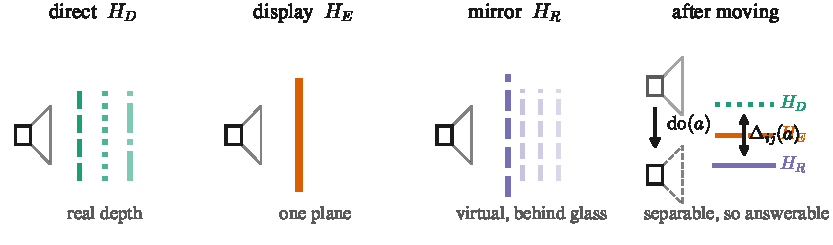
\includegraphics[width=0.92\linewidth]{figures/fig_concept.pdf}
\end{center}
\caption{\textbf{One image, three mechanisms, and what motion reveals.} A real
corridor, the same corridor painted on a display, and its virtual image in a
mirror can be arranged to produce identical pixels at the reference view, so no
single-view method separates them. They differ in the surface a hand would touch,
shown as the coloured plane in each panel. Executing an action makes their
predictions diverge, and the size of that divergence is the separability
$\Delta_{ij}(a)$ of \eqref{eq:separability}.}
\label{fig:concept}
\end{figure}

\section{The decision pipeline}
\label{sec:supp-pipeline}

\begin{figure}[!ht]
\begin{center}
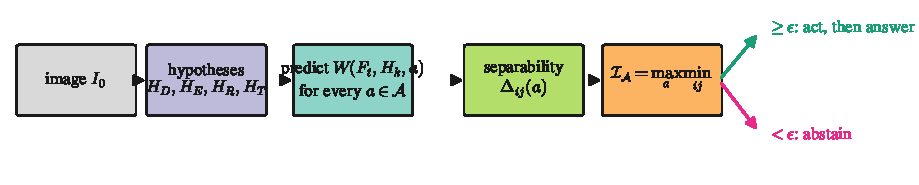
\includegraphics[width=0.96\linewidth]{figures/fig_pipeline.pdf}
\end{center}
\caption{\textbf{How the pieces compose.} Each hypothesis predicts the consequence
of every permitted action \eqref{eq:transition}; pairwise separabilities
\eqref{eq:separability} are formed from those predictions; identifiability is the
best value the action set attains on the weakest contending pair
\eqref{eq:identifiability}. Only when it clears the perceptual threshold is an
action executed and an answer given, and otherwise the system declines
\eqref{eq:abstain}. The whole comparison is made before any motion, which is what
allows abstention in advance of acting.}
\label{fig:pipeline}
\end{figure}

\section{The real-photograph protocol in detail}
\label{sec:supp-protocol}

\begin{figure}[!ht]
\begin{center}
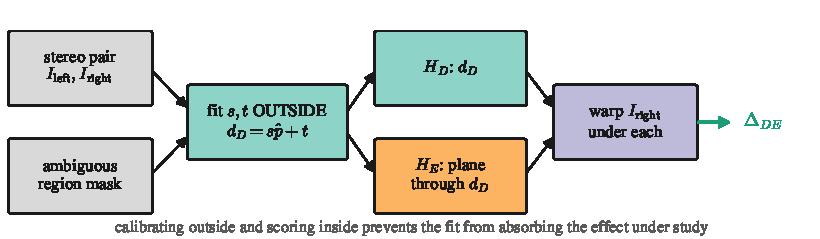
\includegraphics[width=\linewidth]{figures/fig_supp_protocol.pdf}
\end{center}
\caption{\textbf{Construction of the real-data measurement.} Scale and shift are
fitted on the non-ambiguous region and applied inside it, so the two free
parameters are determined where the predictor performs well and cannot absorb the
discrepancy in the region under study. Both hypotheses are then generated from the
predictor's own aligned disparity, never from the reference measurement, and the
right image is warped into the left frame under each. Comparing the two warps
rather than either against the opposite view cancels illumination, sensor noise and
rectification error, which appear identically in both.}
\label{fig:supp-protocol}
\end{figure}

\section{Minimum causal resolving baseline}
\label{sec:supp-mcrb}

For the pair consisting of a direct scene and a static planar display, the motion
required to separate them has a closed form. Under a lateral translation of
baseline $B$, a point at depth $Z$ shifts in the image by approximately $fB/Z$,
where $f$ is the horizontal focal length in pixels, so two points at depths
$Z_1 \neq Z_2$ produce a differential parallax of $fB\,|1/Z_1 - 1/Z_2|$. A static
planar display produces none once the screen-plane homography is compensated.
Requiring the differential parallax to exceed the perceptual threshold $\delta$
gives
\begin{equation}
\label{eq:mcrb}
B_{\min} \;>\; \frac{\delta}{f\left|1/Z_1 - 1/Z_2\right|},
\end{equation}
where $\delta$ coincides with $\epsilon$ whenever the composite distance is
dominated by its motion term. Equation~\eqref{eq:mcrb} is valid only for pure
lateral translation without rotation, a pinhole camera, small baselines satisfying
$B \ll Z$, and this hypothesis pair alone. It does not apply to view-tracked
displays, which no baseline resolves, nor to mirrors, whose virtual scene carries
genuine parallax. These conditions are checked before the expression is evaluated,
so a violated assumption yields a missing prediction rather than a confident wrong
one.

\section{Calibrated deferral and imperfect execution}
\label{sec:supp-noise}

Two studies are reported here: split-conformal deferral on the real benchmark, and the effect of executing a chosen action imperfectly on the synthetic one.

\begin{table}[!ht]
\caption{\textbf{Executing the chosen action imperfectly, paired over $11$ seeds}
($\pm 1$~cm, $\pm 0.5^{\circ}$). Methods that take no action are unchanged at
exactly $0.0\%$, the check that perturbation cannot reach a method that does not
act. Among methods that do act, the hypothesis-blind proxy loses roughly half its
accuracy while ours loses $2.9\%$: actions chosen with a large separability margin
tolerate perturbation, and that margin is what \eqref{eq:maximin} maximises.}
\label{tab:noise}
\begin{center}
\footnotesize
\resizebox{\linewidth}{!}{%
\begin{tabular}{lcccc}
\toprule
\textbf{Method} & \textbf{Clean CEA} & \textbf{Perturbed CEA} & \textbf{Change} & \textbf{$t$} \\
\midrule
Passive multi-view (does not act) & $0.621$ & $0.621$ & $+0.0\%$ & --- \\
Generic NBV proxy   & $0.371$ & $0.192$ & $-48.4\%$ & $-14.05$ \\
Random intervention & $0.409$ & $0.291$ & $-29.0\%$ & $-10.64$ \\
Max-baseline        & $0.502$ & $0.478$ & $-4.7\%$  & $-3.68$ \\
\textbf{Ours}       & $0.560$ & $0.544$ & $\mathbf{-2.9\%}$ & $-3.05$ \\
\bottomrule
\end{tabular}}
\end{center}
\end{table}

\begin{table}[!ht]
\caption{\textbf{Split-conformal selective prediction, $296$ images, $400$
calibration splits per level.} Both signals meet their coverage guarantee at every
level, so neither procedure is broken and the separation appears entirely in
selective risk, which coverage does not constrain. Deferring on confidence tracks
the base rate and then worsens, reaching $76.6\%$; deferring on identifiability
lowers the failure rate at every level, to $54.4\%$ at its best.}
\label{tab:conformal}
\begin{center}
\footnotesize
\resizebox{\linewidth}{!}{%
\begin{tabular}{lccccccc}
\toprule
& & \multicolumn{4}{c}{\textbf{Failure rate among retained images}} & & \\
\cmidrule(lr){3-6}
\textbf{Deferral signal} & \textbf{AUROC} & $\alpha{=}0.2$ & $\alpha{=}0.3$ &
$\alpha{=}0.4$ & $\alpha{=}0.5$ & \textbf{Coverage} & \textbf{Best gain} \\
\midrule
No abstention            & ---     & \multicolumn{4}{c}{$65.2\%$} & --- & --- \\
Confidence (TTA)         & $0.339$ & $64.2\%$ & $65.8\%$ & $69.2\%$ & $76.6\%$ & $5/5$ & $-1.0$ \\
\textbf{Identifiability} & $\mathbf{0.632}$ & $57.9\%$ & $55.1\%$ & $\mathbf{54.4\%}$ & $56.2\%$ & $5/5$ & $\mathbf{-10.8}$ \\
\bottomrule
\end{tabular}}
\end{center}
\end{table}


\section{Per-checkpoint results}
\label{sec:supp-models}

Table~\ref{tab:models} gives the per-checkpoint values summarised in Section~\ref{sec:res-universal}, with parameter counts and family membership.

\begin{table}[!ht]
\caption{\textbf{Twelve published checkpoints, six families, used as released.}
Every checkpoint is fooled on $59.5$--$78.4\%$ of admissible images, and the range
narrows neither with parameter count nor with recency. On every checkpoint the
model's own confidence scores \emph{below chance} at predicting its own failure, so
the usual deferral rule is inverted with respect to what it should track.
Confidence is the better of raw confidence and a four-member test-time-augmentation
ensemble.}
\label{tab:models}
\begin{center}
\footnotesize
\resizebox{\linewidth}{!}{%
\begin{tabular}{llrccc}
\toprule
\textbf{Checkpoint} & \textbf{Family} & \textbf{Params} & \textbf{Fooled} &
\textbf{Confidence AUROC} & \textbf{Ident.\ AUROC} \\
\midrule
DA-V2-Small     & Depth-Anything-V2 & $24.8$M  & $65.2\%$ & $0.344$ & $0.645$ \\
DA-V2-Base      & Depth-Anything-V2 & $97.5$M  & $67.2\%$ & $0.408$ & $0.588$ \\
DA-V2-Large     & Depth-Anything-V2 & $335.3$M & $66.6\%$ & $0.367$ & $0.467$ \\
DA-transparency & Depth-Anything-V2 & $24.8$M  & $\mathbf{59.5\%}$ & $\mathbf{0.234}$ & $0.719$ \\
DA3-Small       & Depth-Anything-3  & $24.8$M  & $76.4\%$ & $0.465$ & $0.479$ \\
DA3-Base        & Depth-Anything-3  & $97.5$M  & $68.2\%$ & $0.362$ & $0.576$ \\
DA3-Large       & Depth-Anything-3  & $410.9$M & $\mathbf{78.4\%}$ & $0.399$ & $0.512$ \\
DepthPro        & DepthPro          & $952.0$M & $65.2\%$ & $0.328$ & $0.659$ \\
MoGe-2          & MoGe-2            & $330.9$M & $62.2\%$ & $0.334$ & $0.642$ \\
Metric3D-Small  & Metric3D          & $37.5$M  & $64.5\%$ & $0.323$ & $0.593$ \\
Metric3D-Large  & Metric3D          & $343.0$M & $67.6\%$ & $0.406$ & $0.593$ \\
UniDepth-v2     & UniDepth          & $353.8$M & $66.2\%$ & $0.295$ & $0.692$ \\
\midrule
\emph{range} & \emph{6 families} & $38\times$ & $59.5$--$78.4\%$ & $0.234$--$0.465$ & $0.467$--$0.719$ \\
\bottomrule
\end{tabular}}
\end{center}
\end{table}

\section{Extended results by architecture family}
\label{sec:supp-family}

Averaging within architecture family confirms that the pattern is not driven by one lineage.

\begin{figure}[!ht]
\begin{center}
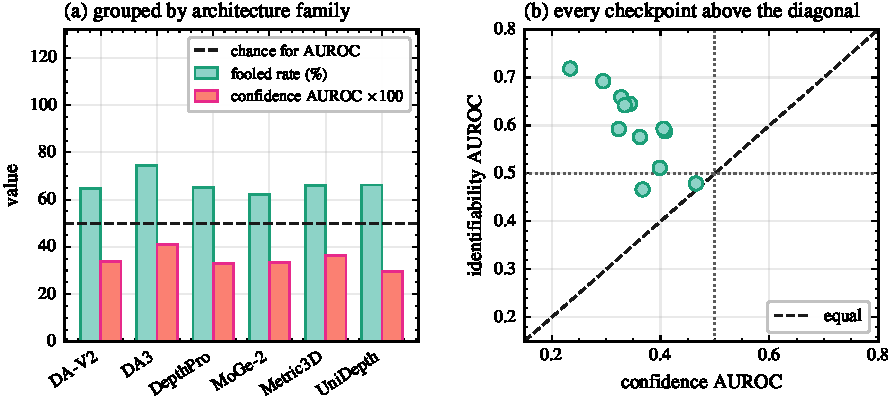
\includegraphics[width=\linewidth]{figures/fig_supp_extended.pdf}
\end{center}
\caption{\textbf{Grouped and paired views of Table~\ref{tab:models}.} (a) Averaged
within each architecture family, the fooled rate sits well above the confidence
AUROC in every family, and every family's confidence average falls below chance.
(b) The same twelve checkpoints plotted against one another: each point lies above
the diagonal, so identifiability exceeds confidence on every checkpoint without
exception, and every point lies to the left of the vertical chance line.}
\label{fig:supp-extended}
\end{figure}

\begin{table}[!ht]
\caption{\textbf{Per-family summary of the twelve checkpoints}, averaged within
family. The pattern of Table~\ref{tab:models} is not driven by one lineage: every
family is fooled on roughly two images in three, and every family's mean confidence
AUROC lies below chance.}
\label{tab:supp-family}
\begin{center}
\footnotesize
\resizebox{\linewidth}{!}{%
\begin{tabular}{lcccc}
\toprule
\textbf{Family} & \textbf{Checkpoints} & \textbf{Mean fooled} &
\textbf{Mean confidence} & \textbf{Mean identifiability} \\
\midrule
Depth-Anything-V2 & $4$ & $64.6\%$ & $0.338$ & $0.605$ \\
Depth-Anything-3  & $3$ & $74.3\%$ & $0.409$ & $0.522$ \\
DepthPro          & $1$ & $65.2\%$ & $0.328$ & $0.659$ \\
MoGe-2            & $1$ & $62.2\%$ & $0.334$ & $0.642$ \\
Metric3D          & $2$ & $66.1\%$ & $0.365$ & $0.593$ \\
UniDepth          & $1$ & $66.2\%$ & $0.295$ & $0.692$ \\
\midrule
\textbf{All}      & $\mathbf{12}$ & $\mathbf{67.3\%}$ & $\mathbf{0.355}$ & $\mathbf{0.597}$ \\
\bottomrule
\end{tabular}}
\end{center}
\end{table}

\section{Learned abstention, summary}
\label{sec:supp-learned}

The table below is the summary referred to from Section~\ref{sec:res-learned}; the section after it expands the leave-one-model-out column to every held-out checkpoint.

\begin{table}[!ht]
\caption{\textbf{Learned abstention.} Folds are split by base scene, so frames of
one scene never span a partition. Success under leave-one-model-out means a
property of the image was learned rather than of one predictor.}
\label{tab:supp-learned}
\begin{center}
\footnotesize
\begin{tabular}{lccc}
\toprule
\textbf{Policy} & \textbf{Grouped CV} & \textbf{Nested CV} & \textbf{Leave-one-model-out} \\
\midrule
\multicolumn{4}{l}{\emph{all 12 checkpoints, 3{,}552 image--model pairs, 68 scenes}} \\
Strongest single feature    & $0.762$ & --- & $0.764$ \\
Logistic regression         & $0.787$ & $0.748$ & $0.808$ \\
\textsc{XGBoost}            & --- & $0.832$ & --- \\
Histogram gradient boosting & $\mathbf{0.832}$ & $\mathbf{0.834}$ & $\mathbf{0.880}$ ($12/12$) \\
\midrule
\multicolumn{4}{l}{\emph{single checkpoint, identical data for all three}} \\
Strongest single feature    & $0.819$ & --- & --- \\
Hand-designed features      & $0.858$ & --- & --- \\
\textbf{Frozen-encoder head} & $\mathbf{0.879}$ & --- & --- \\
\bottomrule
\end{tabular}
\end{center}
\end{table}

\section{Full leave-one-model-out results}
\label{sec:supp-lomo}

The leave-one-model-out protocol of Table~\ref{tab:supp-learned} is expanded to every held-out checkpoint below, together with the regularisation sweep for the frozen-encoder head.

\begin{table}[!ht]
\caption{\textbf{Learned abstention in full.} \emph{Upper block:} every held-out
checkpoint from Table~\ref{tab:supp-learned}. The policy is trained on the other eleven
and evaluated on the one named, which it has never seen; it exceeds the strongest
single feature on all twelve, with a mean margin of $+0.115$ and a minimum of
$+0.051$. \emph{Lower block:} the frozen-encoder head against regularisation
strength. It varies by $0.026$ across three decades and exceeds the hand-designed
feature set ($0.858$) at every setting, so the result reflects the representation
rather than the choice of constant.}
\label{tab:supp-lomo}
\begin{center}
\footnotesize
\resizebox{\linewidth}{!}{%
\begin{tabular}{lccc|lccc}
\toprule
\textbf{Held out} & \textbf{Learned} & \textbf{Baseline} & \textbf{$\Delta$} &
\textbf{Held out} & \textbf{Learned} & \textbf{Baseline} & \textbf{$\Delta$} \\
\midrule
DA-V2-Small     & $0.917$ & $0.819$ & $+0.098$ & DA3-Large      & $0.837$ & $0.731$ & $+0.106$ \\
DA-V2-Base      & $0.901$ & $0.748$ & $+0.153$ & DepthPro       & $0.854$ & $0.721$ & $+0.133$ \\
DA-V2-Large     & $0.930$ & $0.812$ & $+0.118$ & MoGe-2         & $0.899$ & $0.756$ & $+0.143$ \\
DA-transparency & $0.842$ & $0.791$ & $+0.051$ & Metric3D-Small & $0.915$ & $0.787$ & $+0.128$ \\
DA3-Small       & $0.870$ & $0.781$ & $+0.089$ & Metric3D-Large & $0.858$ & $0.750$ & $+0.108$ \\
DA3-Base        & $0.887$ & $0.739$ & $+0.147$ & UniDepth-v2    & $0.849$ & $0.738$ & $+0.111$ \\
\midrule
\multicolumn{8}{c}{\textbf{mean} $\;0.880$ against $0.764$, margin $+0.115$, ahead on $12/12$} \\
\midrule
\multicolumn{8}{l}{\emph{frozen-encoder head: AUROC against regularisation strength $C$, grouped five-fold, one checkpoint}} \\
$C$ & $0.001$ & $0.005$ & $0.020$ & $0.100$ & $0.500$ & $2.000$ & $10.000$ \\
AUROC & $0.869$ & $0.878$ & $\mathbf{0.879}$ & $0.872$ & $0.864$ & $0.859$ & $0.853$ \\
\bottomrule
\end{tabular}}
\end{center}
\end{table}


\section{Per-category behaviour on the illusion benchmark}
\label{sec:supp-category}

The aggregate error ratio quoted in Section~\ref{sec:res-universal} resolves into three categories that behave quite differently.

\begin{table}[!ht]
\caption{\textbf{Admissible images by illusion category.} The penalty for reporting
depicted rather than physical geometry is largest where a display fills the frame,
and the reference measurement inside these regions is close to perfectly planar
while the prediction is not, confirming that the surface is flat and the prediction
is not. This is the per-category detail behind the aggregate quoted in
Section~\ref{sec:res-universal}.}
\label{tab:supp-category}
\begin{center}
\footnotesize
\resizebox{\linewidth}{!}{%
\begin{tabular}{lcccc}
\toprule
\textbf{Category} & \textbf{Images} & \textbf{Error ratio inside/outside} &
\textbf{Fooled} & \textbf{Reference planarity} \\
\midrule
Printed sheet on a table & $97$ & $0.78\times$ & $33\%$ & $0.99$ \\
Poster beside an object  & $104$ & $1.47\times$ & $63\%$ & $0.99$ \\
Monitor filling the frame & $95$ & $\mathbf{2.23\times}$ & $\mathbf{100\%}$ & $0.99$ \\
\midrule
\textbf{All admissible}  & $\mathbf{296}$ & $\mathbf{1.42\times}$ & $\mathbf{65.2\%}$ & $\mathbf{0.989}$ \\
\bottomrule
\end{tabular}}
\end{center}
\end{table}

\section{Second dataset with ordinal supervision}
\label{sec:supp-layered}

The second dataset supplies ordinal relations between point pairs rather than dense depth, and carries a per-point layer index authored independently of this work.

\begin{table}[!ht]
\caption{\textbf{LayeredDepth validation, $299$ images, $306{,}874$ annotated point
pairs.} Accuracy is split by the benchmark authors' own per-point layer index, a
label written independently of this work that shares no machinery with any measure
defined here. Both architectures are markedly worse on points visible only through
a transparent surface, and the penalty is larger for the model with more
parameters. The ambiguity this paper formalises is therefore recognised by an
independent annotation and independently predicts failure, on supervision that is
ordinal rather than dense and on a dataset collected by a different group.}
\label{tab:supp-layered}
\begin{center}
\footnotesize
\resizebox{\linewidth}{!}{%
\begin{tabular}{lccccc}
\toprule
\textbf{Checkpoint} & \textbf{Single-layer acc.} & \textbf{Multi-layer acc.} &
\textbf{Gap} & \textbf{Ordinal acc.\ (first surface)} & \textbf{Ordinal acc.\ (through glass)} \\
\midrule
DA-V2-Small & $0.848$ & $0.737$ & $\mathbf{+0.111}$ & $0.847$ & $0.784$ \\
DepthPro    & $0.843$ & $0.669$ & $\mathbf{+0.175}$ & $0.842$ & $0.741$ \\
\bottomrule
\end{tabular}}
\end{center}
\end{table}

\section{Choosing where to look}
\label{sec:supp-viewpoint}

Fifty-five non-video scenes offer three or more camera positions of the same
static content. Video scenes are excluded because their frames differ by what is
displayed rather than by where the observer stands, so treating them as an action
set would count a change of stimulus as a change of viewpoint.

\begin{table}[!ht]
\caption{\textbf{Viewpoint selection on real photographs}, $12$ checkpoints over
$55$ scenes, lower is better on both columns. Selecting by
\eqref{eq:evidence-selection}, the viewpoint at which some hypothesis best accounts
for the observed view, lowers the error inside the ambiguous region by $31.6\%$
against a random choice and wins on every checkpoint. Error inside the region is
the primary column because it depends on no other part of the image; the fooled
rate is reported alongside for continuity with the rest of the paper.}
\label{tab:supp-viewpoint}
\begin{center}
\footnotesize
\begin{tabular}{lcc}
\toprule
\textbf{Viewpoint chosen by} & \textbf{Error inside region} & \textbf{Fooled} \\
\midrule
first frame, no choice          & $0.0695$ & $49.2\%$ \\
uniformly at random             & $0.0610$ & $48.7\%$ \\
the predictor's own confidence  & $0.0450$ & $47.1\%$ \\
\textbf{best-explained observation} \eqref{eq:evidence-selection} & $\mathbf{0.0417}$ & $\mathbf{44.1\%}$ \\
\midrule
\multicolumn{3}{l}{\emph{ahead of a random choice on $12/12$ checkpoints by error, $9/12$ by fooled rate}} \\
\bottomrule
\end{tabular}
\end{center}
\end{table}

A note on the comparison with published methods. The benchmark's authors release
both their data and a trained checkpoint. The datasets carry an explicit
Apache-2.0 licence and are used here accordingly; the checkpoint carries no licence
field on its model repository, no \texttt{LICENSE} file on either default branch of
the source repository, and no licence statement in its README, all checked on
2026-08-29. A direct comparison against it is therefore deferred until those terms
are stated, rather than made under unclear ones.

\section{Metric definitions}
\label{sec:supp-metrics}

The metrics used throughout are defined below.

\begin{table}[!ht]
\caption{\textbf{The reported metrics.} $\hat{H}$ is the predicted mechanism,
$H^\star$ the true one, $p(H_k)$ the posterior mass on hypothesis $k$, $\tau$ the
confidence threshold of Section~\ref{sec:belief}, and $y_{\mathrm{id}} = 0$ marks a
case no permitted action resolves. CEA and committed accuracy are reported together
because the first penalises excessive caution and the second rewards it.}
\label{tab:supp-metrics}
\begin{center}
\footnotesize
\begin{tabular}{llp{6.0cm}}
\toprule
\textbf{Metric} & \textbf{Definition} & \textbf{Question it answers} \\
\midrule
CEA & $P(\hat{H} = H^\star)$ & how often the mechanism is named correctly, abstention counted as an error \\
Committed acc. & $P(\hat{H} = H^\star \mid \text{answered})$ & when an answer is given, how often it is right \\
Abstention rate & $P(\text{abstain})$ & how often an answer is withheld \\
FPCR & $P(\max_k p(H_k) > \tau \mid y_{\mathrm{id}} = 0)$ & how often a confident answer is given where none is warranted \\
Ident.\ AUROC & predicted against true resolvability & whether unresolvable cases are recognised \\
Normalised regret & chosen against best available action & whether a near-optimal intervention was selected \\
Motion cost & translation plus weighted rotation & how much movement the decision required \\
\bottomrule
\end{tabular}
\end{center}
\end{table}

\section{Scope and limitations}
\label{sec:supp-limits}

Four limits bound what the reported numbers establish, and each is visible in the
results rather than inferred.

\textbf{The synthetic identifiability AUROC is degenerate by construction.} On the
synthetic benchmark the computation producing the identifiability prediction is the
same one producing the ground-truth label, so the value of $1.000$ in
Table~\ref{tab:phase1} carries no information about the method's accuracy. It is
reported only as a contrast against the classifiers, which reach $0.505$ and
$0.748$ on identical scenes, and no claim rests on its absolute value.

\textbf{Abstention is not unconditionally safe under encoder noise.} The clean
configuration reaches a false physical certainty rate of $0.000 \pm 0.000$ across
all $11$ seeds, but the noisy-encoder ablation reaches $0.008 \pm 0.026$: one seed
in eleven produces a false certainty. The correct statement is therefore
``zero in $10$ of $11$ seeds under encoder noise'', not ``zero''.

\textbf{Real-data evidence rests on stereo, which supplies a single action.} A
calibrated pair gives $|\mathcal{A}| = 1$, so \eqref{eq:identifiability} reduces to
one term and the selection results of Table~\ref{tab:phase2} cannot be tested on
this data. Evaluating the choice of intervention on real photographs requires a
multi-view or controllable-camera capture, which the datasets used here do not
provide.

\textbf{One checkpoint runs in a degraded configuration.} UniDepth-v2 has no
optimised attention kernel for the available hardware and falls back to a slower
path, so its numbers in Table~\ref{tab:models} are a lower bound on the released
model rather than a tuned comparison. It is retained because excluding a checkpoint
on the basis of its result would bias the sweep.

\section{Reproducibility}
\label{sec:supp-repro}

All synthetic results are averaged over $11$ seeds with the benchmark redrawn per
seed, so the reported intervals reflect the data-generating process rather than
model-side noise alone. Splits are formed by base scene throughout, in both the
synthetic benchmark and the learned-policy protocols, so variants or frames of a
single scene never span a partition. Every depth checkpoint is used exactly as
released and nothing is trained or tuned on any evaluation set. Each checkpoint's
output convention is verified against reference stereo disparity before use, since
the attribute conventionally named \texttt{predicted\_depth} carries metric depth
in some families and inverse depth in others. One checkpoint, UniDepth-v2, runs
without its optimised attention kernel on the available hardware, so its numbers
should be read as a lower bound on the released model rather than a tuned
comparison.
